\documentclass[border=10pt]{standalone}
\usepackage{tikz}\usepackage{amsmath}\usetikzlibrary{arrows.meta}
\begin{document}
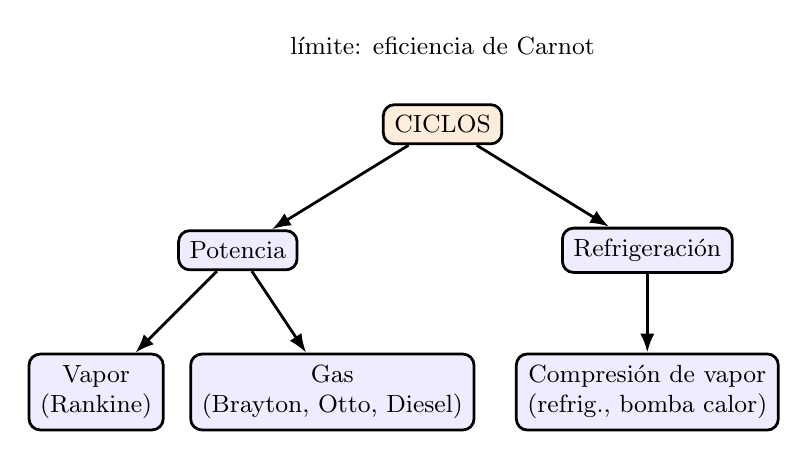
\begin{tikzpicture}[font=\small,>={Latex[length=2.4mm]},
  nd/.style={draw,line width=1pt,rounded corners,fill=blue!7,align=center,inner sep=4pt}]
  \node[nd,fill=orange!14] (c) at (0,0) {CICLOS};
  \node[nd] (pot) at (-2.6,-1.6) {Potencia};
  \node[nd] (ref) at (2.6,-1.6) {Refrigeración};
  \node[nd] (vap) at (-4.4,-3.4) {Vapor\\(Rankine)};
  \node[nd] (gas) at (-1.4,-3.4) {Gas\\(Brayton, Otto, Diesel)};
  \node[nd] (vcr) at (2.6,-3.4) {Compresión de vapor\\(refrig., bomba calor)};
  \draw[->,line width=1pt] (c)--(pot); \draw[->,line width=1pt] (c)--(ref);
  \draw[->,line width=1pt] (pot)--(vap); \draw[->,line width=1pt] (pot)--(gas);
  \draw[->,line width=1pt] (ref)--(vcr);
  \node at (0,1.0){\small límite: eficiencia de Carnot};
\end{tikzpicture}
\end{document}
